\documentclass[11pt]{article}
\usepackage[utf8]{inputenc}
\usepackage{geometry}
\usepackage{amsfonts}
\usepackage{hyperref}
\usepackage{enumitem}
\usepackage{graphicx}
\usepackage{tabularx}
\usepackage{amsmath}
\usepackage{xcolor}
\usepackage{array}
\usepackage{amsmath}
\usepackage{amssymb}
\usepackage{algorithm}
\usepackage{algorithmic}
\usepackage{graphicx}



\title{
    \textbf{CSE634: Algorithms in Robot Planning} \\ \vspace*{-5pt}
    \textbf{\large{Assignment-1}}
}

\author{Akanksha Singal (2021008)}
\date{\today}

\geometry{a4paper, left=20mm, right=20mm, top=20mm, bottom=20mm}


\begin{document}
\maketitle

\section*{Question-1}
In the Charging Station Placement Problem, we have discussed the variant FindNCS that finds the minimum number and placement of the charging stations, given a battery threshold. We have also discussed the Max-3-CNF problem and a randomized approximation algorithm for solving Max-3-CNF. Design a randomized approximation algorithm for solving the FindNCS problem. Hint: Formulate the FindNCS problem as the Max-k-CNF problem.

\subsection*{Solution}

\subsection*{Problem: FINDNCS}

Given: A directed graph \( G = (V, E) \) with a set of potential charging stations \( \text{CS} \subseteq V \) and a battery threshold (number of transitions) \( d \)
\newline
Objective: To minimize the number of charging stations \( ncs \) and find the charging station vertices \( \text{MCS} = \{v_{c_1}, \ldots, v_{c_{ncs}}\} \) from \( \text{CS} \) such that at least one vertex in \( \text{MCS} \) is reachable from any vertex \( v \in V \) by traversing a path of length at most \( d \).


\subsection*{Max-$k$-CNF Problem}

Given: A Boolean formula $\phi$ in conjunctive normal form (CNF), where each clause contains at most $k$ literals.
\newline
Objective: Find a truth assignment to the variables that satisfies the maximum number of clauses. 
    
\subsection*{Formulating FindNCS as Max-$k$-CNF}
The FindNCS problem aims to place the minimum number of charging stations such that each node within the network is covered based on a given battery threshold. We can model this as a Max-$k$-CNF problem:

\begin{itemize}
\item \textbf{Variables/Literals:} 
\newline
For every vertex \( v \in CS \) (the set of potential charging station locations), we define a Boolean variable $x_v$ where:
\[
x_v = 
\begin{cases}
1 & \text{if a charging station is placed at location } v, \\
0 & \text{otherwise.}
\end{cases}
\]
\textbf{Variables/Literals:} \( x_v \in \{0, 1\} \) for all \( v \in CS \).

\item \textbf{Clauses:} 

For each vertex \( u \in V \) (all vertices in the graph), we define a clause \( C_u \) as follows:

Let \( S(u) \) be the set of vertices in \( CS \) that are reachable from \( u \) within \( d \) steps (i.e., there exists a path from \( u \) to \( v \) of length at most \( d \)).

The clause \( C_u \) is then defined as:

\[
C_u = \bigvee_{v \in S(u)} x_v
\]

This clause ensures that for vertex \( u \), at least one of the reachable potential charging stations within the battery threshold is active (i.e., has a charging station placed).

\item \textbf{Formulating the problem as a Max-k-CNF instance:} 


The overall formula \( \Phi \) is the conjunction of all clauses:

\[
\Phi = \bigwedge_{u \in V} C_u
\]

Each clause \( C_u \) is a disjunction (logical OR) of variables and represents a constraint that must be satisfied for \( u \) to be covered.

The clauses are in Conjunctive Normal Form (CNF), and each clause contains at most \( k \) literals, where \( k \) is the maximum size of \( S(u) \).

\end{itemize}

\subsection*{Randomized Approximation Algorithm}
Based on the formulation above we design randomized approximation algorithm to maximise the number of clauses as True. We can derive this algorithm from the Max-k-SAT problem. 

\begin{algorithm}
    \caption{Randomized Approximation Algorithm for FindNCS}
    \begin{algorithmic}[1]
        \STATE \textbf{INPUT: } Graph $G = (V, E)$, battery threshold $d$, set of potential charging stations $CS$
        \STATE \textbf{OUTPUT: } Subset $MCS$ - approximate minimum number of Charging Stations
        \STATE Assign each literal $x_v$ to $1$ (place a charging station at $v$) independently with probability $p$
        \STATE $MCS \leftarrow { v \in V \mid x_v = 1 }$
        \STATE \textbf{Return} $MCS$
    \end{algorithmic}
\end{algorithm}

\subsection*{Explanation}
Random assignment of $x_v = 1$  with probability $p$ , and $x_v = 0$  with probability $1 - p$. If we assign $p = 1/2$ we get a 1/2 - approximation algorithm. Other ways of solving Maximum satisfiability problem is using derandomisation and Integer Program and Linear Program for Maximum Satisfiability. 

\subsection*{Approximation Ratio}
Approximation algorithm with probability 1/2 gives an assignment that satisfies at least half of the number of clauses. The proof can be found \href{https://www.cse.iitb.ac.in/~rgurjar/CS602_2020/LectureNotes/lec19-2.pdf}{\textcolor{blue}{here}} on page 1 and 2.

\section*{Question 2}
We are given a directed graph \( G = (V, E) \) on which each edge \( (u, v) \in E \) has an associated value \( r(u, v) \) which is a real number in the range \( 0 \leq r(u, v) \leq 1 \) that represents the reliability of a communication channel from vertex \( u \) to vertex \( v \). We interpret \( r(u, v) \) as the probability that the channel from \( u \) to \( v \) will not fail, and we assume that these probabilities are independent. Give an efficient algorithm to find the most reliable path
between two given vertices.

\subsection*{Solution}

\textbf{Given:}
\begin{itemize}
    \item \textbf{Graph Definition:} \( G = (V, E) \)
    \begin{itemize}
        \item \( V \): Set of vertices 
        \item \( E \): Set of edges
    \end{itemize}
    
    \item \textbf{Edge Probability:} Each edge \( (u, v) \in E \) has an associated probability value \( r(u, v) \).
    \begin{itemize}
        \item \( r(u, v) \) is a real number in the range \([0, 1]\).
    \end{itemize}
    
    \item \textbf{Probability Interpretation:}
    \begin{itemize}
        \item \( r(u, v) \) represents the \textbf{probability that the channel from node \( u \) to node \( v \) }\textbf{does not fail}.
        \item A higher \( r(u, v) \) indicates a more reliable channel.
    \end{itemize}
    
    \item \textbf{Independence:} The probabilities \( r(u, v) \) for each edge are \textbf{independent} of each other.
\end{itemize}


\textbf{To find:} most reliable path between two given vertices

\subsection*{Proposed Algorithm }
In order to find the most reliable path, we can interpret the probabilities as cost of the edge where the cost is between \([0, 1]\). Our goal now is to maximize the cost between any two given vertices. This would ensure that the entire path is the most reliable. 

\begin{figure}[h]
    \centering
    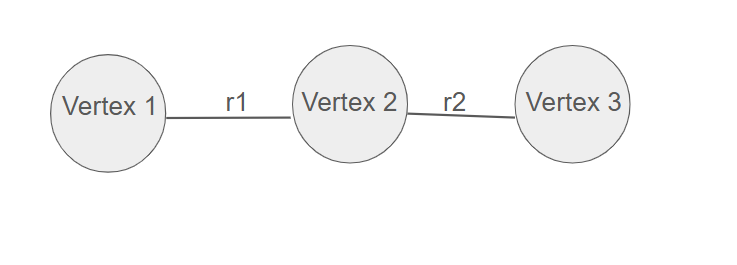
\includegraphics[width=0.5\textwidth]{arp_q2.png}
    \caption{Example Graph}
    \label{fig:example}
\end{figure}

Consider the path from \textbf{Vertex 1} to \textbf{Vertex 3}, which goes through \textbf{Vertex 2}:

\begin{itemize}
    \item Edge \((1, 2)\) has reliability \( r_1 \).
    \item Edge \((2, 3)\) has reliability \( r_2 \).
\end{itemize}

The total probability of the path from \textbf{Vertex 1} to \textbf{Vertex 3} is:
\[
\text{Total reliability} = r_1 \times r_2
\]

To find the most reliable path from \textbf{Vertex 1} to \textbf{Vertex 3}, we need to maximize this product:

\begin{itemize}
    \item If \( r_1 \) is the maximum probability for the edge from \textbf{Vertex 1} to \textbf{Vertex 2}.
    \item If \( r_2 \) is the maximum probability for the edge from \textbf{Vertex 2} to \textbf{Vertex 3}.
\end{itemize}

Then, the product \( r_1 \times r_2 \) is maximized, making this path the most reliable. The multiplication rule applies because the edge probabilities are independent.
To ensure the maximum reliability of a path, we must select edges with the highest possible reliability values.

Now to maximize the probability values represented as cost of the edges in the graph we can use modified Dijkstra's algorithm or modified Bellman ford algorithm to maximize the cost between any two vertices. 

We will assume that the directed graph does not have cycles. We can additionally add preprocessing step before the algorithm to remove circles and only keep the edges with the maximum weights in the graph.



\begin{algorithm}
\caption{Most Reliable Path Using Modified Bellman-Ford}
\begin{algorithmic}[1]
\STATE \textbf{INPUT}: Directed Graph $G = (V, E)$, $r(u, v)$ for each $(u, v) \in E$, source vertex $s$, and destination vertex $t$
\STATE \textbf{OUTPUT}: Most reliable path from $s$ to $t$ in terms of maximum reliability

\STATE Initialize reliability $\text{cost}(v) \leftarrow \infty$ for each $v \in V$
\STATE Set $\text{cost}(s) \leftarrow 0$
\STATE Initialize predecessor $\text{pred}(v) \leftarrow \text{None}$ for each $v \in V$

\FOR{$i = 1$ to $|V| - 1$}
    \FOR{each edge $(u, v) \in E$}
        \IF{$\text{cost}(u) + r(u, v) > \text{cost}(v)$}
            \STATE $\text{cost}(v) \leftarrow \text{cost}(u) + r(u, v)$
            \STATE $\text{pred}(v) \leftarrow u$
        \ENDIF
    \ENDFOR
\ENDFOR
\FOR{each edge $(u, v) \in E$}
    \IF{$\text{cost}(u) + w(u, v) > \text{cost}(v)$} \STATE
        \textbf{Report} that a positive cycle exists that can increase the cost indefinitely
        \RETURN \textbf{False} 
    \ENDIF
\ENDFOR

\STATE Construct the path from $s$ to $t$ using the $\text{pred}$ array
\STATE Output the path

\end{algorithmic}
\end{algorithm}

\subsection*{Explanation}
We are first iterating for $V - 1$ times, in each iteration for each edge we check if the reliability to any vertex v is greater from any other vertex u. If the reliability is greater then we update the value at v and update the predecessor. Lines 14-19 are for checking cycles in the graph.


\subsection*{Time Complexity}
The time complexity of this algorithm is same as Bellman Ford's algorithm that is \(O(VE) \),
\end{document}